\section{404 pages}

Il sito non ha sviluppato una pagina specifica per gestire il caso in cui 
l'utente richieda una pagina specifica che non esista. È possibile trovare 
due diverse pagine 404: la figura \ref{fig:404-academy} illustra il 
risultato se viene cercato un articolo inesistente della \textit{Academy} 
e la figura \ref{fig:404-support} illustra il risultato se viene cercato 
un contenuto inesistente della pagina \textit{Supporto}. Queste pagine sono 
molto grezze e non forniscono delle informazioni utili all'utente. 
L'utilizzo del codice di errore 404 può essere omesso, in quanto rappresenta 
un tecnicismo che non è utile per l'utente. Anche il link per tornare alla 
homepage presente nella figura \ref{fig:404-support} rappresenta un 
riferimento per poter tornare ad un punto familiare per l'utente, tuttavia 
rappresenta anche uno svantaggio: se l'utente ha raggiunto tale pagina 
inesistente tramite il \textit{deep linking}, far tornare indietro 
l'utente significherebbe farlo uscire dal sito. Nella figura 
\ref{fig:404-academy} è possibile vedere che la pagina 404 non viene 
gestita bene: a parte la frase ironica, tutti testi dei menù, dei bottoni 
e del footer non vengono caricati. Questo può causare un forte 
disorentamento per l'utente. Tra l'altro, essendo la sezione di articoli 
di apprendimento, quindi frequentata soprattutto da utenti neofiti, non 
contribuisce a mantenere un buon livello di qualità.

\begin{figure}[H]
  \centering
  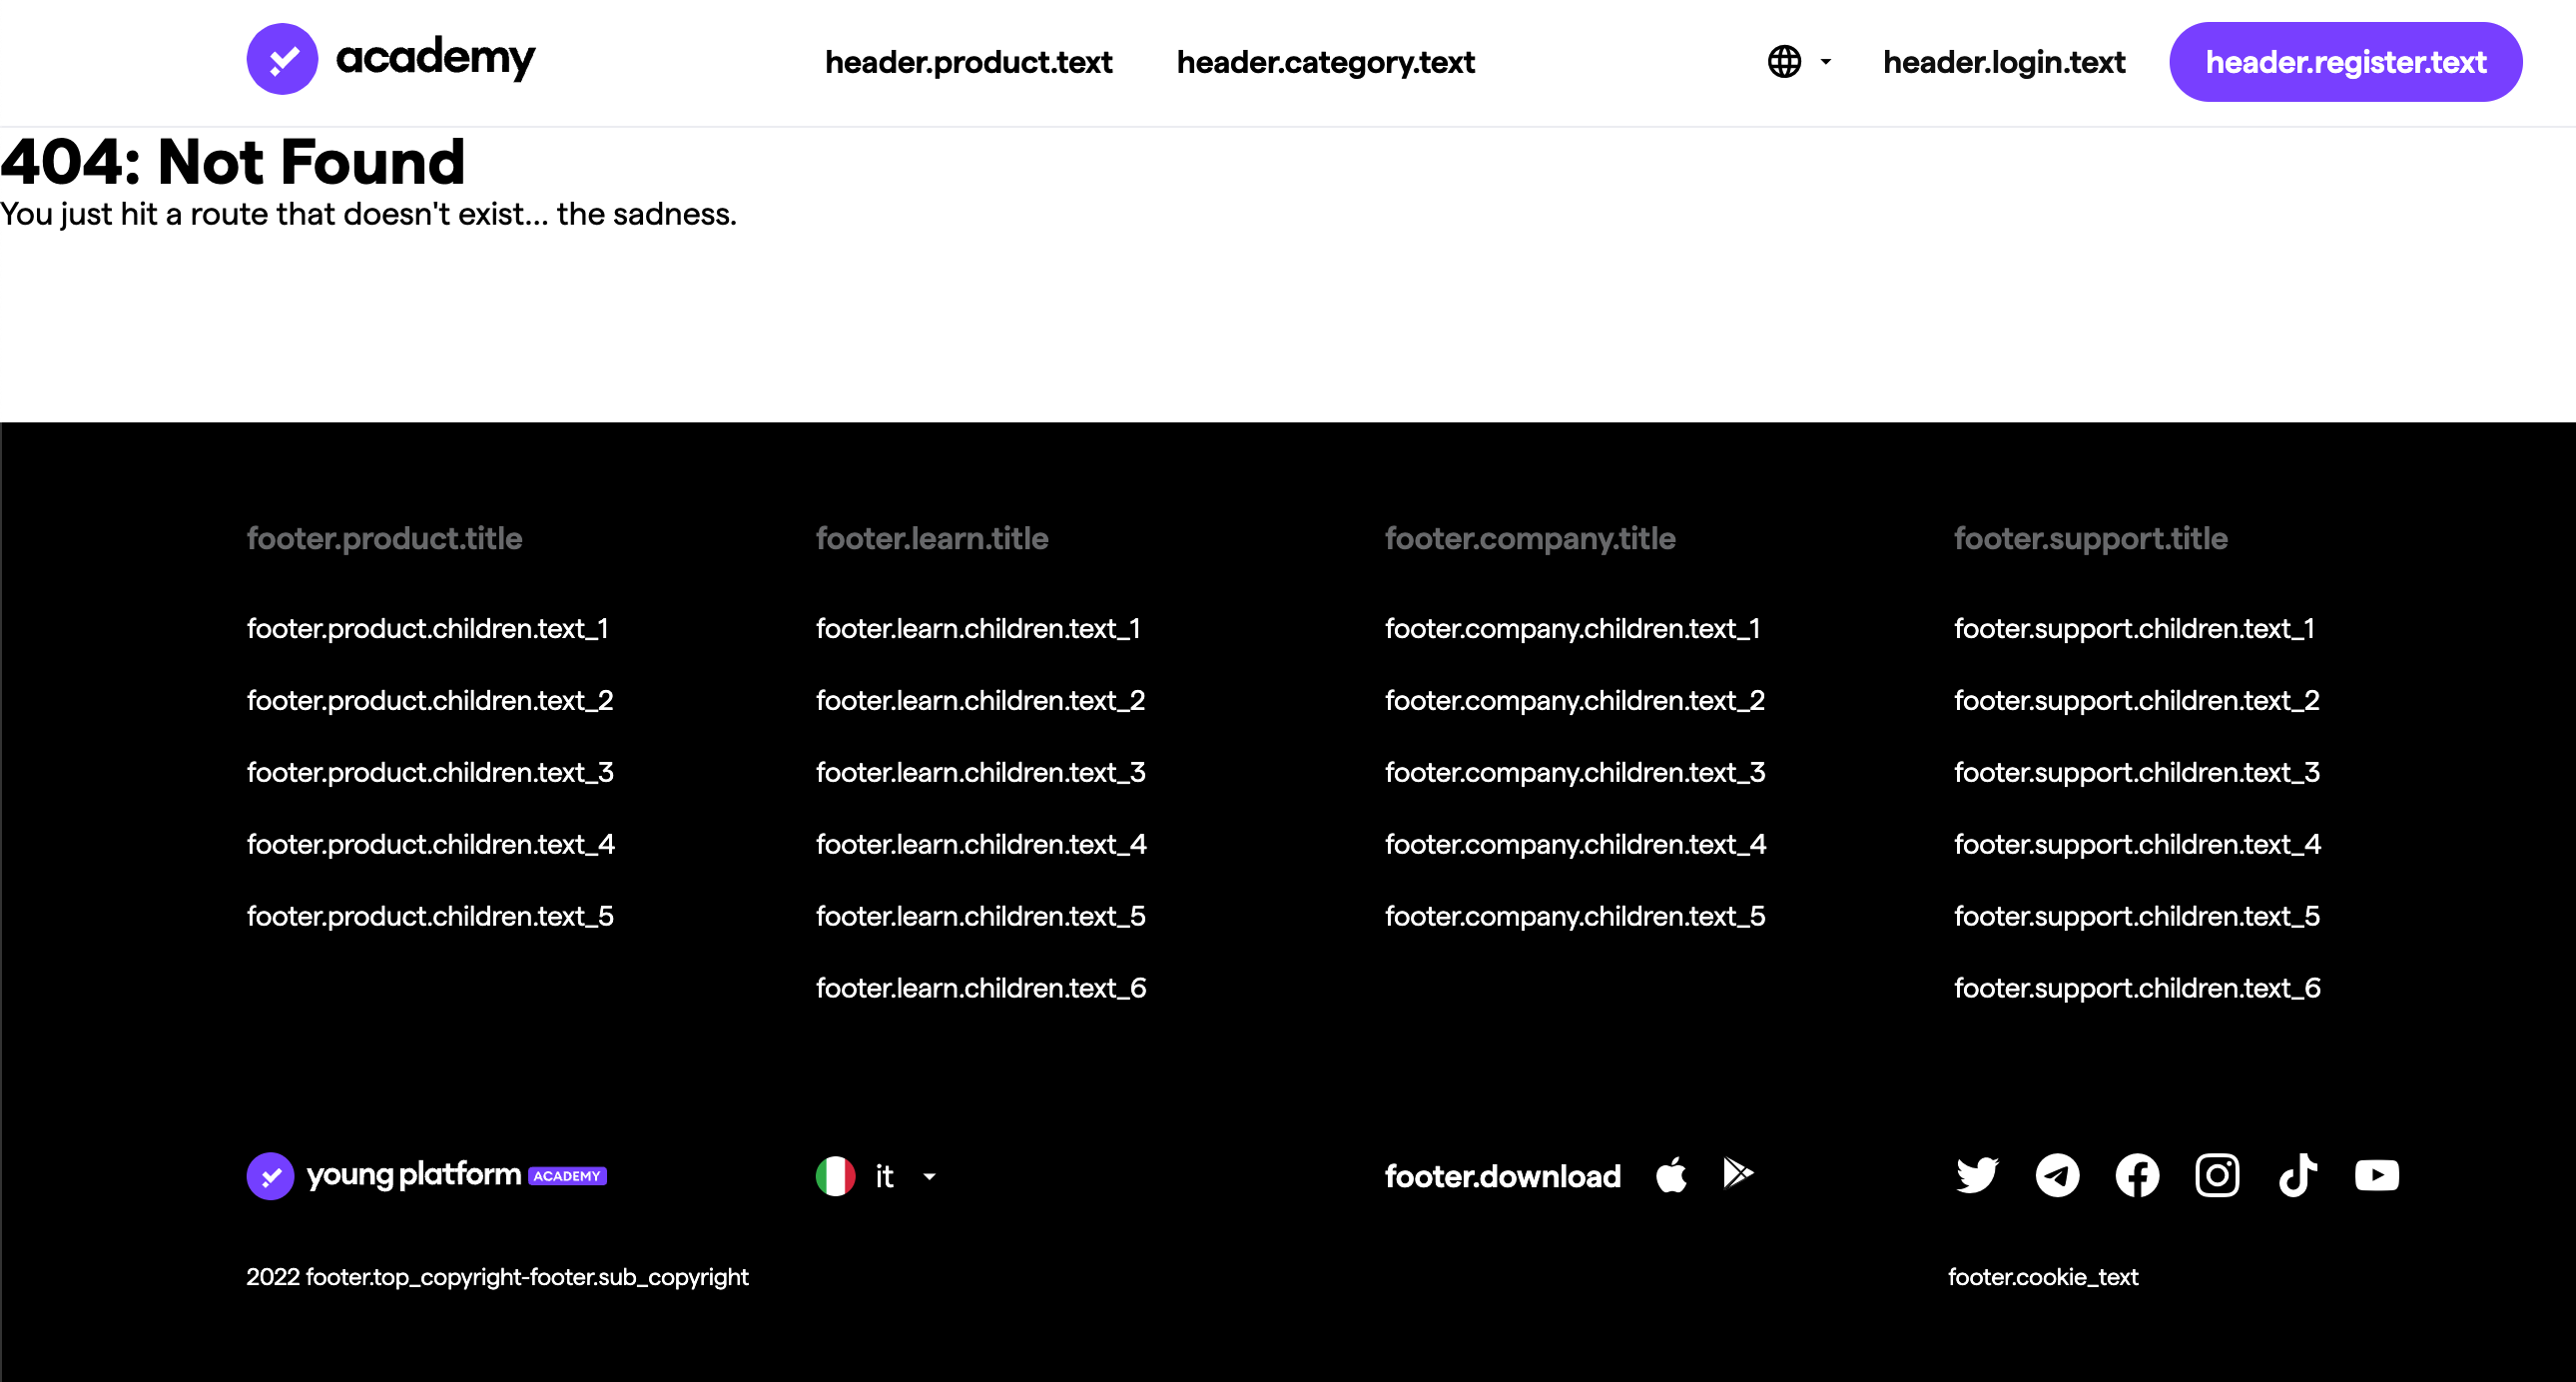
\includegraphics[width=0.80\textwidth]{res/images/404-academy.png}
  \caption{Pagina 404 che si presenta se non viene trovato un articolo 
  della \textit{Academy}.}
  \label{fig:404-academy}
\end{figure}

\begin{figure}[H]
  \centering
  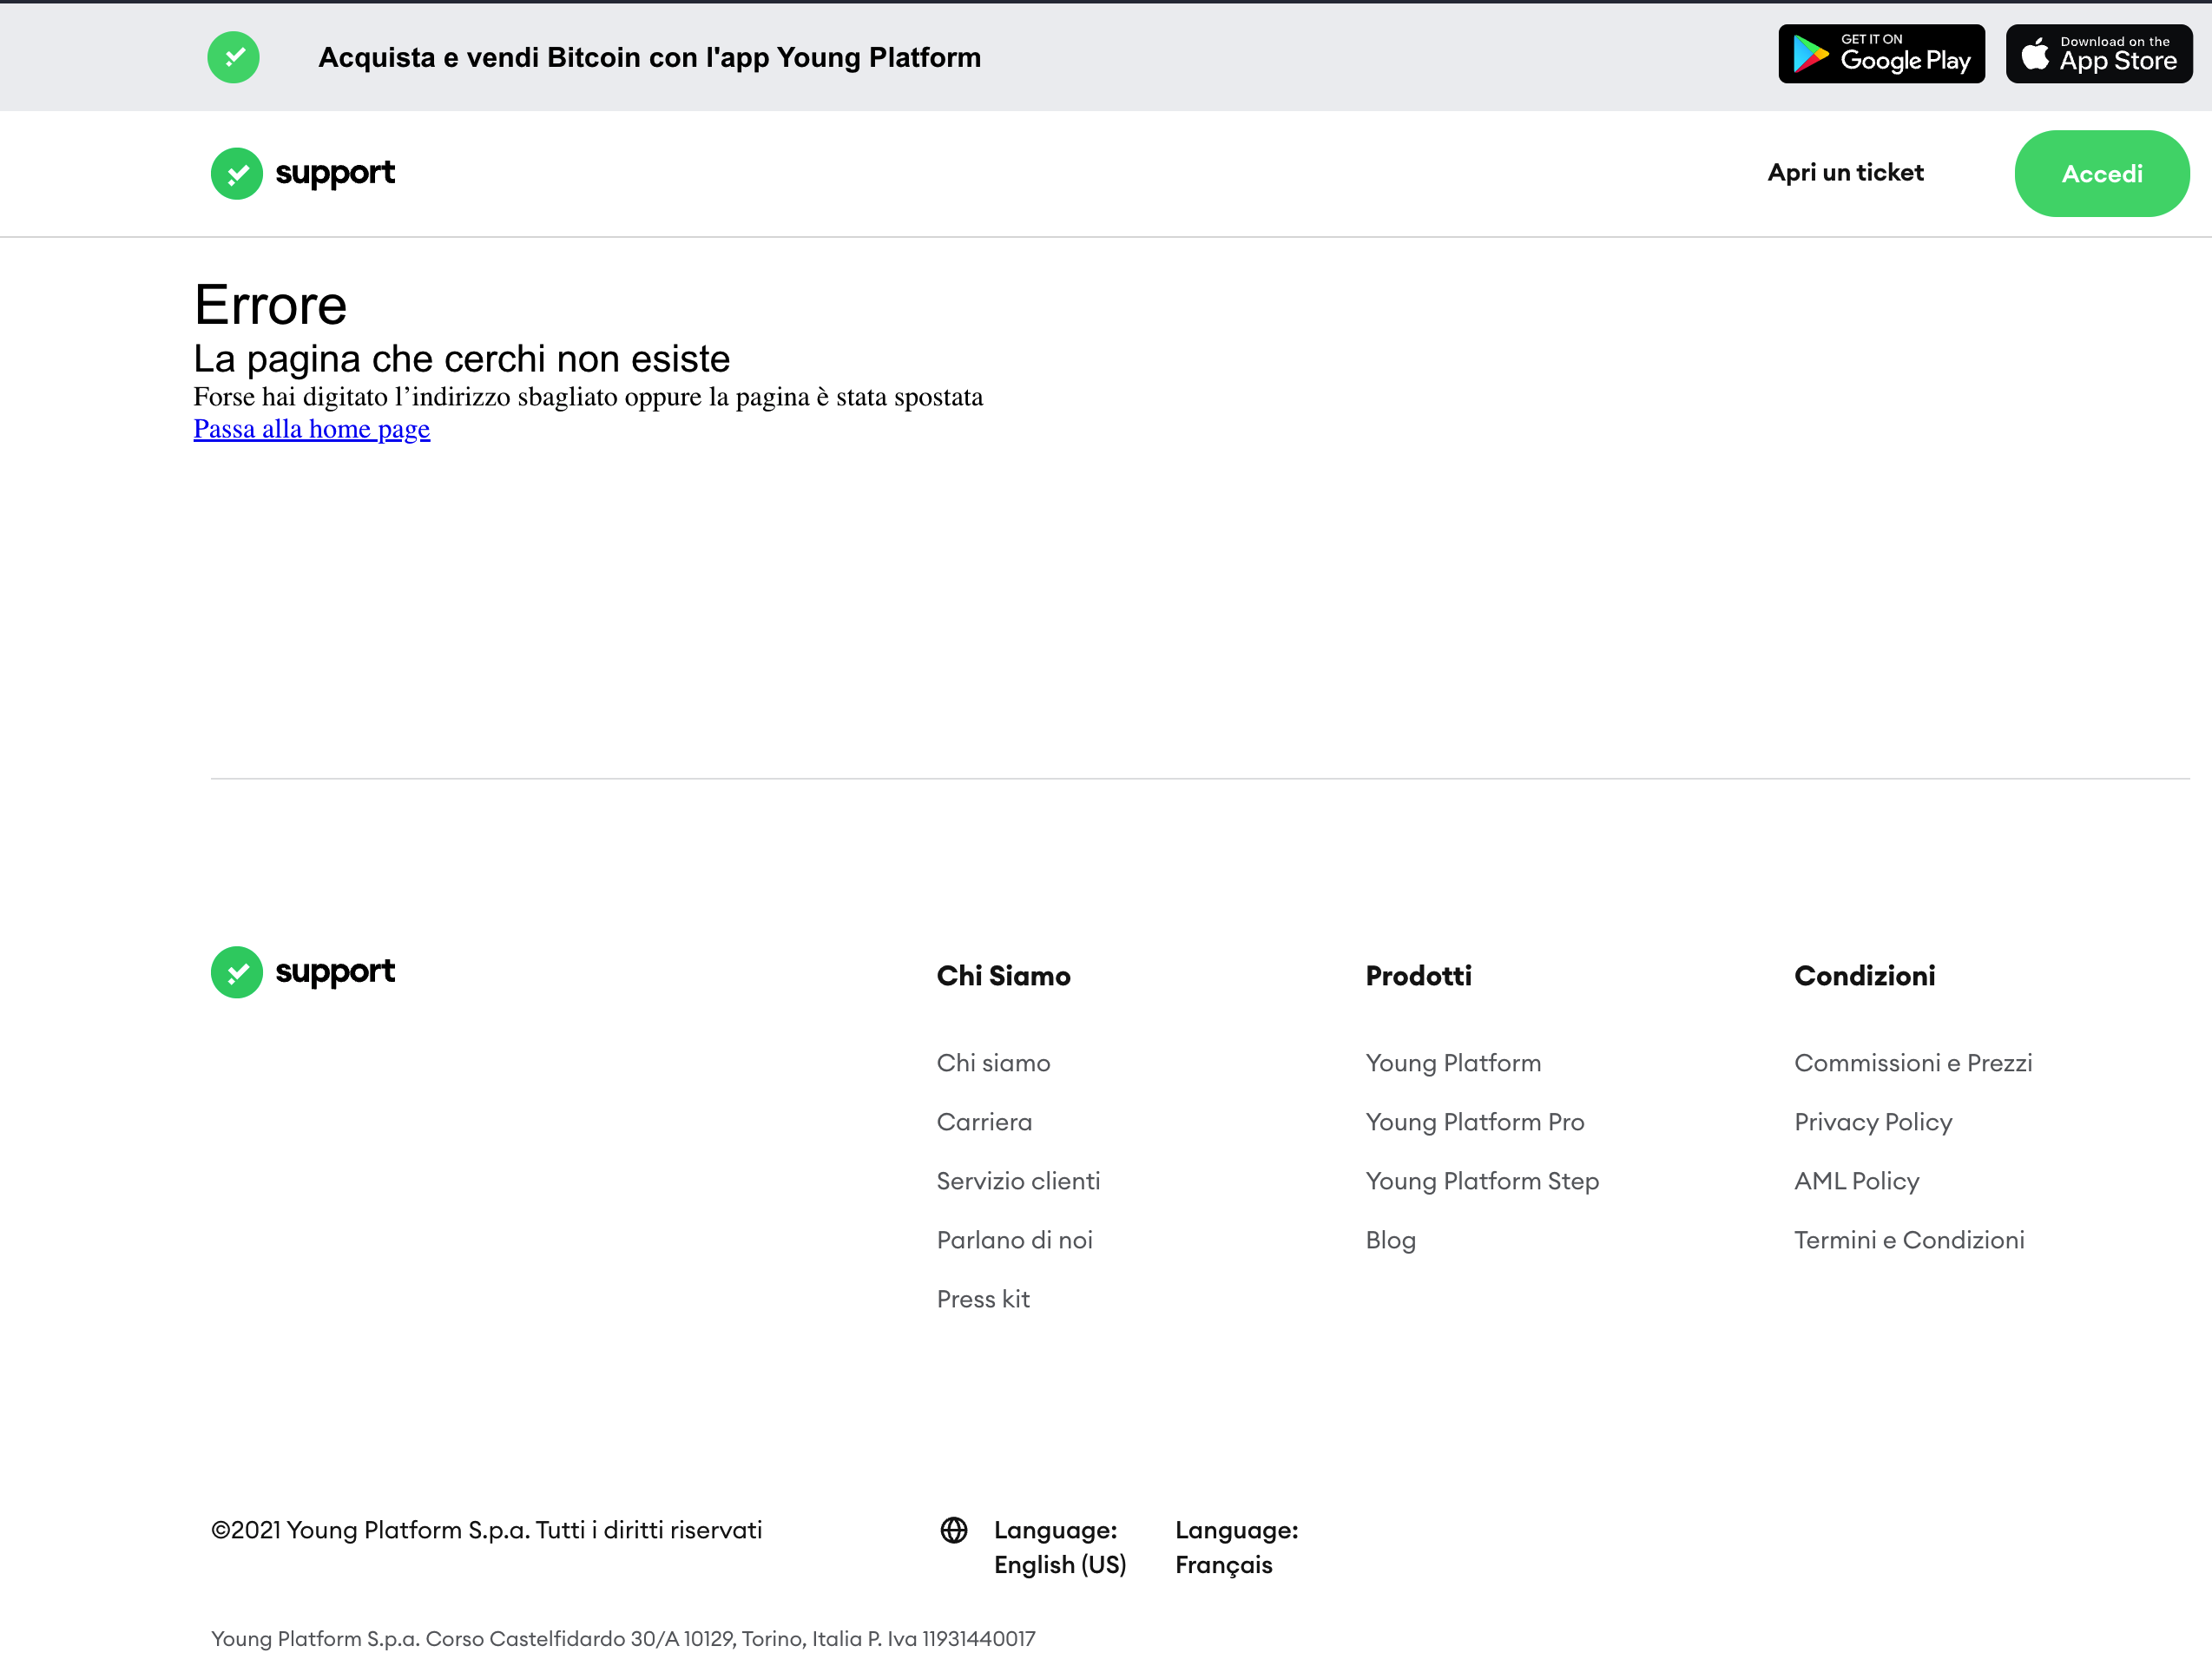
\includegraphics[width=0.80\textwidth]{res/images/404-support.png}
  \caption{Pagina 404 che si presenta se si cerca un contenuto non presente 
  nella pagina \textit{Supporto}.}
  \label{fig:404-support}
\end{figure}